%%%%%%%%%%%%%%%%%%%%%%%%%%%%%%%%%%%%%%%%%%%%%%%%%%%%%%%%%%%%%%%%%%%%%%%%%%%%%%%%
%2345678901234567890123456789012345678901234567890123456789012345678901234567890
%        1         2         3         4         5         6         7         8

\documentclass[letterpaper, 10 pt, conference]{ieeeconf}  % Comment this line out
                                                          % if you need a4paper
%\documentclass[a4paper, 10pt, conference]{ieeeconf}      % Use this line for a4
                                                          % paper

\IEEEoverridecommandlockouts                              % This command is only
                                                          % needed if you want to
                                                          % use the \thanks command
\overrideIEEEmargins
% See the \addtolength command later in the file to balance the column lengths
% on the last page of the document



% The following packages can be found on http:\\www.ctan.org
%\usepackage{graphics} % for pdf, bitmapped graphics files
%\usepackage{epsfig} % for postscript graphics files
%\usepackage{mathptmx} % assumes new font selection scheme installed
%\usepackage{times} % assumes new font selection scheme installed
\usepackage{amsmath} % assumes amsmath package installed
\usepackage{amssymb}  % assumes amsmath package installed
\usepackage{amsfonts}
\usepackage{graphicx}
\usepackage{caption}
\usepackage{subcaption}
\usepackage{array}

\title{\LARGE \bf
Feed forward networks: The delta rule and back propagation
}

%\author{ \parbox{3 in}{\centering Huibert Kwakernaak*
%         \thanks{*Use the $\backslash$thanks command to put information here}\\
%         Faculty of Electrical Engineering, Mathematics and Computer Science\\
%         University of Twente\\
%         7500 AE Enschede, The Netherlands\\
%         {\tt\small h.kwakernaak@autsubmit.com}}
%         \hspace*{ 0.5 in}
%         \parbox{3 in}{ \centering Pradeep Misra**
%         \thanks{**The footnote marks may be inserted manually}\\
%        Department of Electrical Engineering \\
%         Wright State University\\
%         Dayton, OH 45435, USA\\
%         {\tt\small pmisra@cs.wright.edu}}
%}

\author{ Federico Baldassarre, Diego Gonz\'alez Mor\'in, Lucas Rod\'es Guirao \\
KTH Royal Institute of Technology
}


\begin{document}



\maketitle
\thispagestyle{empty}
\pagestyle{empty}


%%%%%%%%%%%%%%%%%%%%%%%%%%%%%%%%%%%%%%%%%%%%%%%%%%%%%%%%%%%%%%%%%%%%%%%%%%%%%%%%
%\begin{abstract}


%\end{abstract}


%%%%%%%%%%%%%%%%%%%%%%%%%%%%%%%%%%%%%%%%%%%%%%%%%%%%%%%%%%%%%%%%%%%%%%%%%%%%%%%%
\section{INTRODUCTION}
Feed Forward Networks are introduced in this lab, which further explores some of their applications (e.g. \emph{classification}, \emph{function approximation} and \emph~{generalization}). In this regard, it first begins using only single-layer networks, where the \emph~{delta rule} is used as a training method. Later, it generalized to multi-layer networks and the \emph{generalized delta rule}.

The focus of this lab is not on the implementation but rather on the understanding of the covered topics. We note that almost all the MATLAB code is provided by the lab tutorial.

\section{CLASSIFICATION WITH ONE LAYER PERCEPTRON}

\subsection{Generating the training data}

We generate a data matrix of dimension $d \times N$, where $d$ is the number of features and $N$ is the number of samples. In addition it also generates the associated targets (since we examine a binary classifier, we only use two different labels). In this regard we define two different functions. On the one hand, \texttt{sepdata} generates linear separable data. On the other hand In particular, we implement a function \texttt{nsepdata} which generates non linear-separable data.

\subsection{Implementation of the Delta rule}
%
Suppose we have the input $\textbf{x} = (x_1, \dots, x_d)^T$, the output $\textbf{t} = (t_1, \dots, t_p)$ and the associated weights. For instance, $w_{j,i}$ connects $x_i$ and $t_j$ for all $i \in {1,\dots,d}$ and $j \in \{1,\dots,p\}$. Given the input, the perceptron tries to estimate the output by finding the appropriate weights such that

$$
\sum_{k=1}^d w_{j,k} x_k \approx t_j.
$$

Hence, we can define the error obtained in the estimation as 

$$
\varepsilon = \frac{1}{2} \Big(\sum_k w_{j,k} x_k - t_j\Big)^2 \qquad (1)
$$

We can update the weights using the error measure. In particular we obtain the direction in which the error increases the less (opposite of Gradient) and add it to the weights as

$$
w_{j,i}^{new} = w_{j,i}^{old} + \eta \Delta w_{j,i},
$$

where 
$$
\Delta w_{j,i} = -\frac{\partial \varepsilon}{\partial w_{j,i}} = -x_i\Big(\sum_k w_{j,k} x_k - t_j\Big).
$$


%

Alternatively, we can update the matrix of weights using

$$
\Delta W = -\eta (W\textbf{x} - \textbf{t})\textbf{x}^T.
$$

If we were to consider the contributions from several training patterns, suppose from the whole epoch, we would rather use the update equation

$$
\Delta W = -\eta (WX - T){X}^T,
$$

where $X$ is $d\times n$ and $T$ is $p \times n$, being $n$ the number of training patterns. \\

In our case, we have an input with two features, i.e. $\textbf{x} = (x_1, x_2)^T$ and one scalar output $t \in \{-1,1\}$. In other words, we have that $d=2$ and $p=1$. Thus we have a 2:1 network, which means that $W$ is $1\times 2$ matrix. Furthermore, we used $N=200$ samples. In the following we present the results from applying the delta rule on two different sets, i.e. linear separable and non linear-separable illustrated in Fig. \ref{fig:s} and Fig. \ref{fig:ns}, respectively.\\


\begin{figure*}
    \centering
    \begin{subfigure}[b]{0.49\textwidth}
        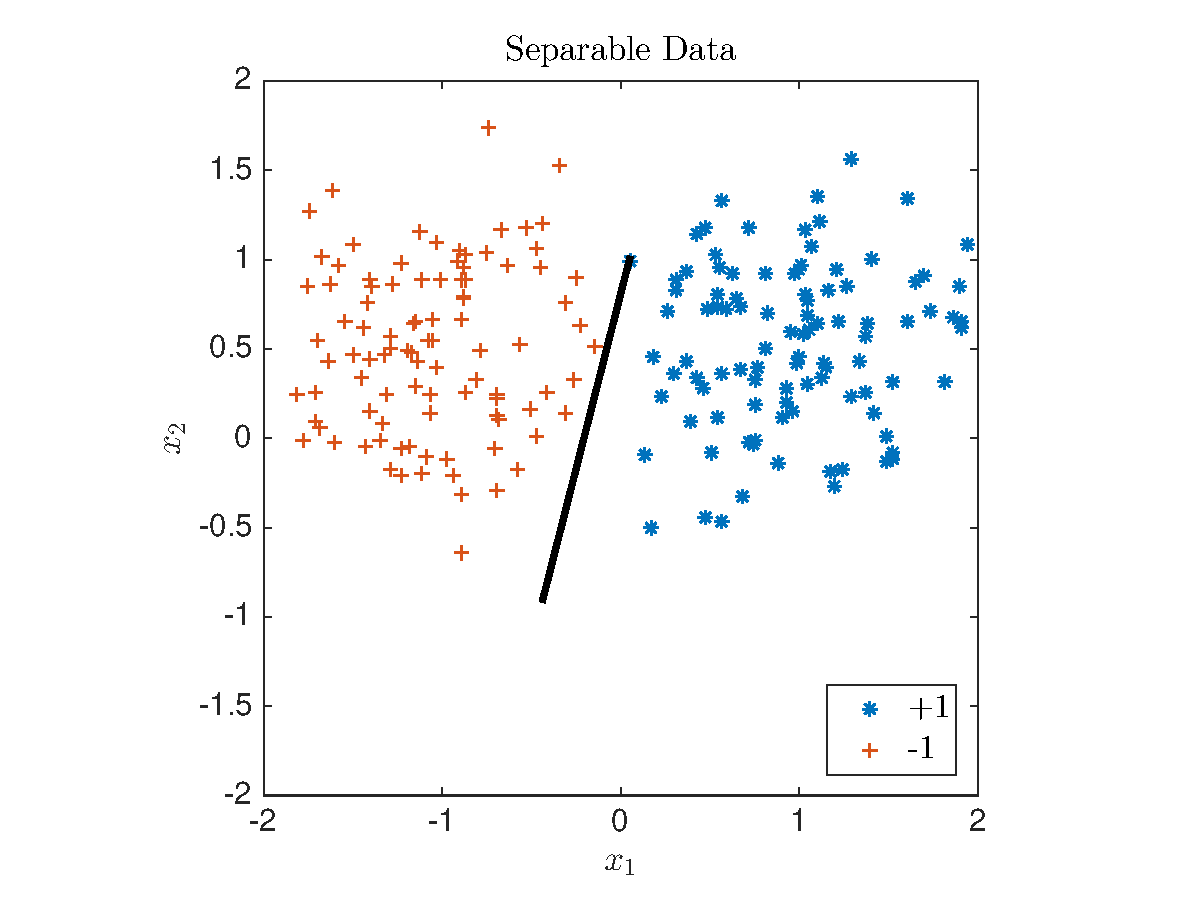
\includegraphics[width=\textwidth]{separable}
        \caption{Single Layer perceptron works fine when the data is linearly separable.}
        \label{fig:s}
    \end{subfigure}
    \begin{subfigure}[b]{0.49\textwidth}
        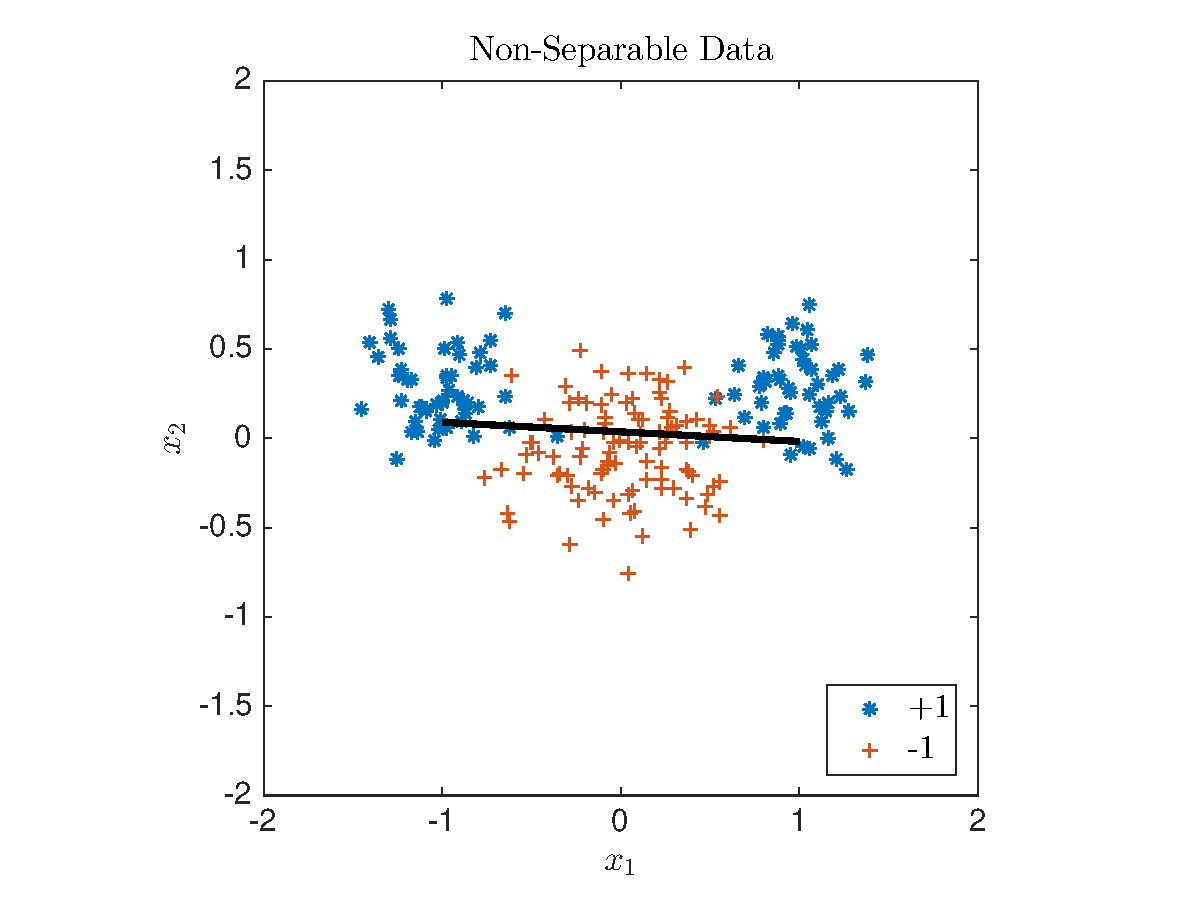
\includegraphics[width=\textwidth]{nonseparable}
        \caption{Single layer perceptron performs very poorly when the data is not separable.}
        \label{fig:ns}
    \end{subfigure}
    \caption{Decision boundary estimated using a single layer perceptron for different sets of data. In particular we have binary-labeled data (+1, -1).}
\end{figure*}


\section{CLASSIFICATION WITH THE TWO LAYER PERCEPTRON}

In order to tackle more complex training sets, such as the one shown in Fig. \ref{fig:ns}, we need to increase the complexity of the model. This is achieved by using the so-called \emph{generalized Delta rule}. A first approach could be to add hidden layers between the input and outpu layers. However, This would still preserve the linear dependence between inputs and outputs. To overcome this, we use a non-linear transfer function, often denoted by $\varphi$, at each neuron in the hidden layers. As highlighted in the lab tutorial, this function is chosen so that it is easily derived like

$$
\varphi(x) = -\frac{e^{-x}}{1+e^{-x}},
$$

such that its derivative is given by

$$
\varphi'(x) = \frac{[1+\varphi(x)][1-\varphi(x)]}{2}.
$$

The generalized delta rule consists of three parts. It first applies the forward pass, which is responsible of computing the activities at each node. This procedure is done starting from the input layer and ending at the output layer. Next, the backward pass is done. It starts at the output layer and obtains the error signals $\delta$ at each node. Finally, using the activities and the error signals the weights are updated. For this example, we will asume we have one hidden layer, with a certain amount of neurons leading to the NN structure $d : M : p$ (In our case $d=2$ and $p=1$). Let us briefly detail the key equations in these three different steps.

\subsection{The forward pass}
Consider $x_i$ as the input feature at the $i$:th node at the input layer. We define the summed input signal to the $j$:th node of the hidden layer as

$$
h_j^\ast = \sum_i w_{j,i} x_i,
$$

and the output signal at this node as 
$$h_j = \varphi(h_j^\star).$$ 

The same occurs with the output layer, namely we have for the $k$:th node at the output layer that $o_k = \varphi(o_k^\star)$ being $o_k^\ast = \sum_j v_{k,j} h_j$.

In MATLAB, we can wisely use tha matrix notation to increase the efficiency. In particular we use

$$
H = \varphi(WX) \quad, \quad O = \varphi(VH),
$$

where each column of $H$ contains a vector $h \in \mathbb{R}^M$ ($M$ being the number of neurons in the hidden layer). However, we make sure that at the end we add a row to $H$ which stands for the bias term in the hidden layer.

\subsection{The backward pass and weight update}
The basic idea here is the same as in (1), however we now aim at finding the weights such that

$$
\varepsilon = \frac{1}{2} \Big(\sum_k \varphi(o_k^\ast) - t_k\Big)^2 \qquad (2)
$$

is minimized. In this regard, for the output layer we have that

$$
\Delta v_{k,j} = - \frac{\partial \varepsilon}{\partial v_{k,j}} = -h_j \delta_k^{(o)}
$$

and for the hidden layer we have that

$$
\Delta w_{j,i} = - \frac{\partial \varepsilon}{\partial w_{j,i}} = -x_i \delta_j^{(h)},
$$ 

where we have defined the error signals as 

$$
\delta_k^{(o)} = (o_k - t_k) \cdot \varphi'(o_k^\ast)
$$

and

$$
\delta_j^{(h)} = \bigg( \sum_k v_{k,j} \delta_k^{(o)} \bigg) \cdot \varphi'(h_j^\ast).
$$

\subsection{All together}
Finally we join all the different steps and build a Neuron Network with one hidden layer with 4 neurons, i.e. with a NN structure $2 : 4 : 1$. Fig. \ref{f:2} illustrates the results obtained, in particular it shows the MSE at each epoch. As expected, the error tends to decrease as the number of epochs increases. Bear in mind, however, that the error is obtained using only the training data, meaning that having zero error might lead to overfitting and thus poor generalization on unseen data. We note that the error curve approaches zero more rapidly in the linear-separable data (it is a more simple model).

\begin{figure*}
    \centering
    \begin{subfigure}[b]{0.49\textwidth}
        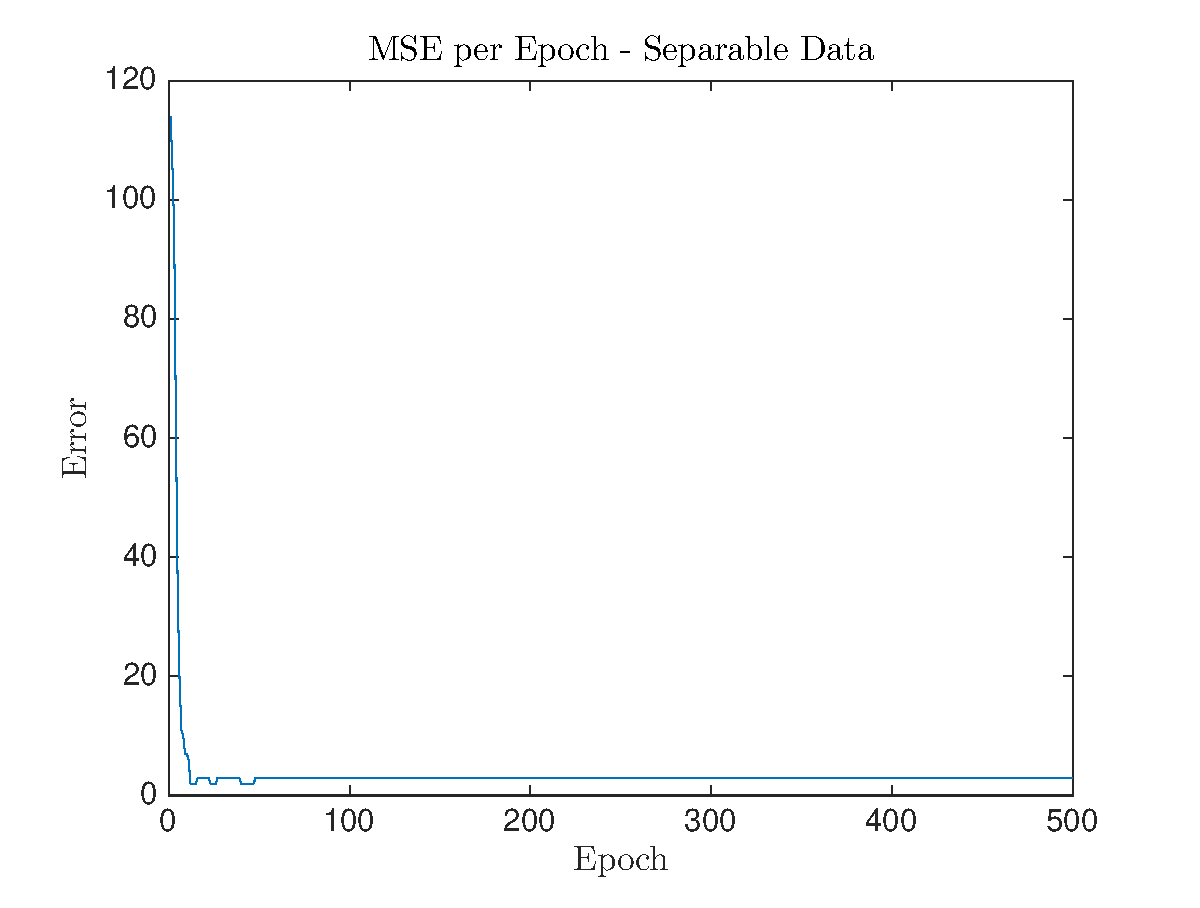
\includegraphics[width=\textwidth]{backprops}
        \caption{Multilayer perceptron with linearly separable data. The MSE curve rapdily decreases to close-to-zero values.}
        \label{fig:s}
    \end{subfigure}
    \begin{subfigure}[b]{0.49\textwidth}
        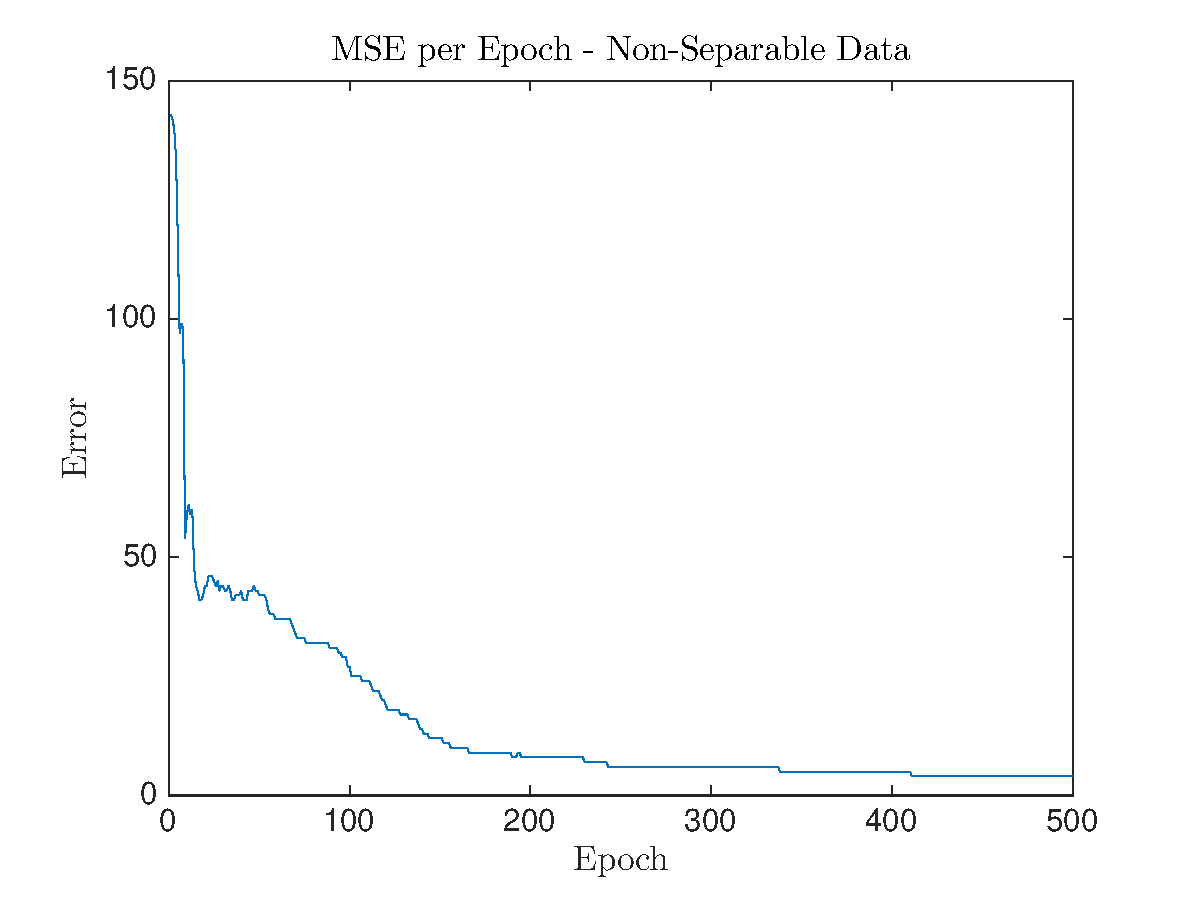
\includegraphics[width=\textwidth]{backpropns}
        \caption{Multilayer perceptron with non linearly-separable data. It takes more epochs to reach similar error values as with separable data.}
        \label{fig:ns}
    \end{subfigure}
    \caption{MSE curve for two different cases.}
    \label{f:2}
\end{figure*}

\subsection{The encoder problem}
In this problem a hour glass shaped topology is used in the Neural Network. This means that the number of neurons in the hidden layer is much lower than the number of neurons in the input and output layers. In particular, the input and output are always the same which forces the network to find a compact representation of the input (output) data in the hidden layer. 

In our example we use an eight-sized binary input, i.e. $\textbf{x} \in \mathbb{R}^8$. However, we only use it to encode 8 different symbols, which could instead be encoded using only 3 digits. In particular the possible input vectors consist on vectors containing only $-1$ coefficients and one coefficient equal to $1$. For this purpose we will use a 8:3:8 network. Fig. \ref{f:enc} illustrates the corresponding MSE. 


\begin{figure}[h]
\centering
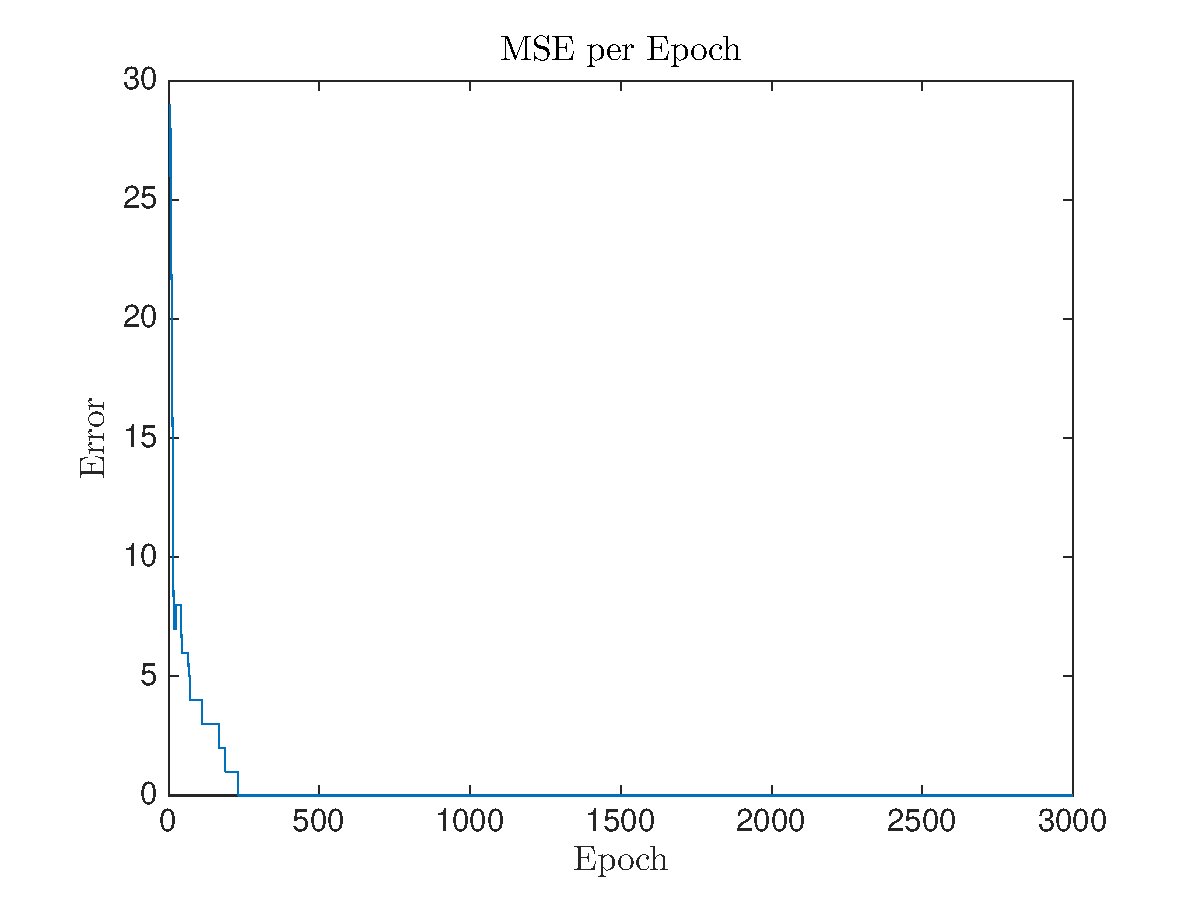
\includegraphics[scale=0.4]{encoder}
\caption{Mean square error of the encoder.}
\label{f:enc}
\end{figure}




Table \ref{t:1} shows the values of the hidden layer. In particular, we have first used the function sign to obtain $-1$/$1$ values and then we have replaced $-1$ for $0$. We observe that the compression in the results shown in the table is perfect, since there is no input data that are compressed to the same value.


\begin{table}
\begin{center}
\begin{tabular}{ |c|c|c|  }
\hline
 \multicolumn{3}{|c|}{Encoder results} \\
 \hline
In & Hidden & Output \\
 \hline
 $1$ & $101$ & $1$ \\
 $2$ & $010$ & $2$ \\
 $3$ & $001$ & $3$ \\
 $4$ & $011$ & $4$ \\
 $5$ & $000$ & $5$ \\
 $6$ & $110$ & $6$ \\
 $7$ & $111$ & $7$ \\
 $8$ & $100$ & $8$ \\
 \hline
\end{tabular}
\end{center}
\caption{Results of the hidden layer}
 \label{t:1}
\end{table}

\section{FUNCTION APPROXIMATION}
In this section we will use the network to approximate an arbitrary continuous function. For this purpose we will use a two layer network (one hidden layer). The function to approximate is given as inputs and outputs for the network. The function is bivariate and is given by

$$
f(x,y) = e^{-(x^2+y^2)/10}-0.5
$$

In Fig. \ref{f:3} we illustrate the results of the function estimation for different number of neurons in the hidden layer. In particular we observe that $2$ seems to perform poorly while $6$ neurons seems to be a good choice. 
\begin{figure*}
    \centering
    \begin{subfigure}[b]{0.85\textwidth}
        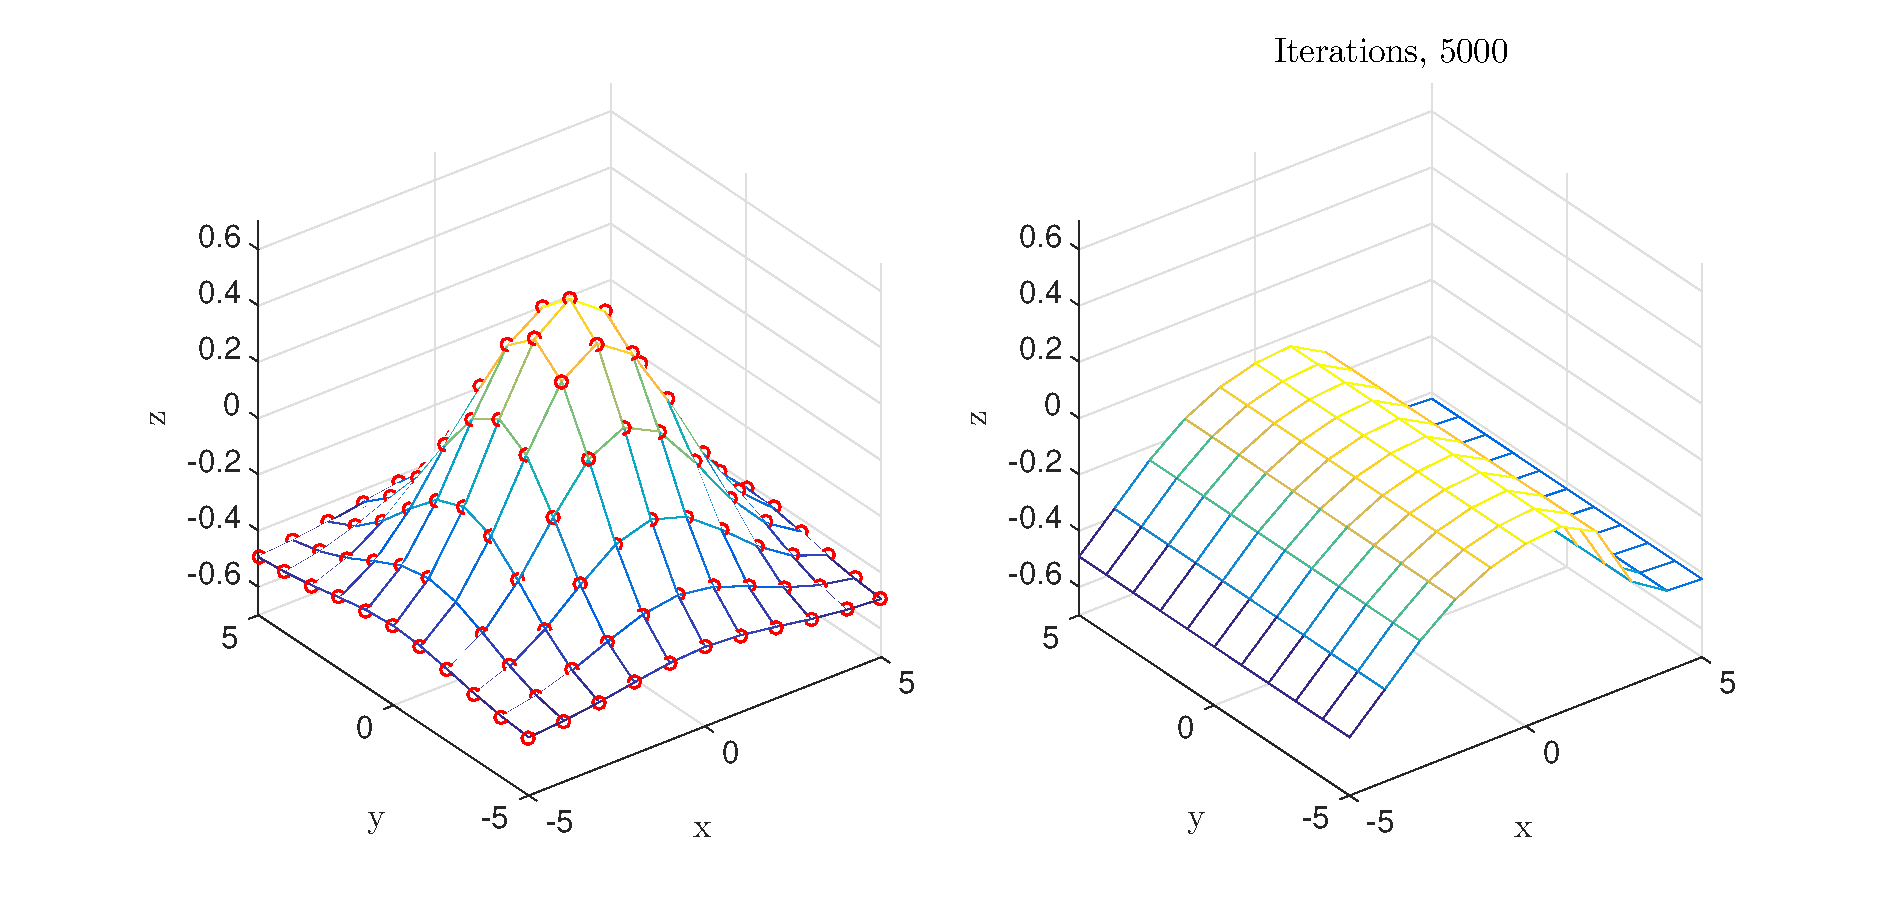
\includegraphics[width=\textwidth]{function_approximation_2}
        \caption{2 neurons in the hidden layer.}
        \label{fig:31}
    \end{subfigure}


    \begin{subfigure}[b]{0.85\textwidth}
        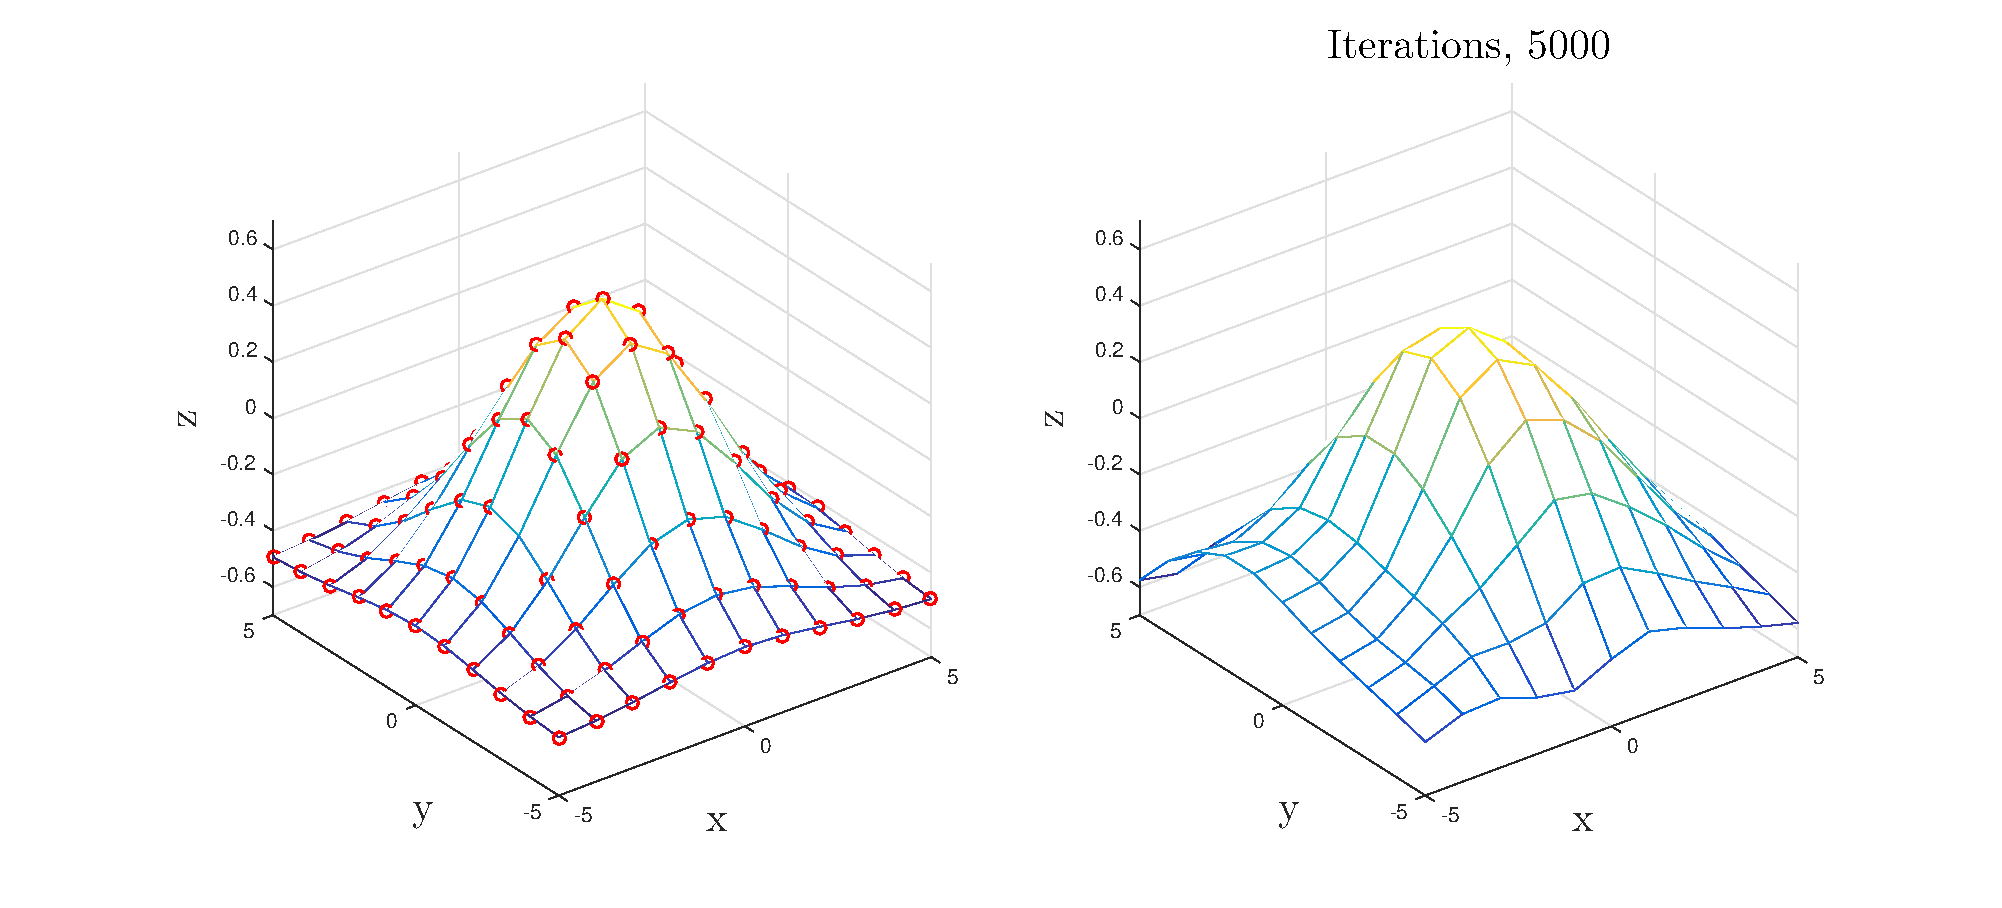
\includegraphics[width=\textwidth]{function_approximation_6}
        \caption{6 neurons in the hidden layer.}
        \label{fig:32}
    \end{subfigure}


    \begin{subfigure}[b]{0.85\textwidth}
        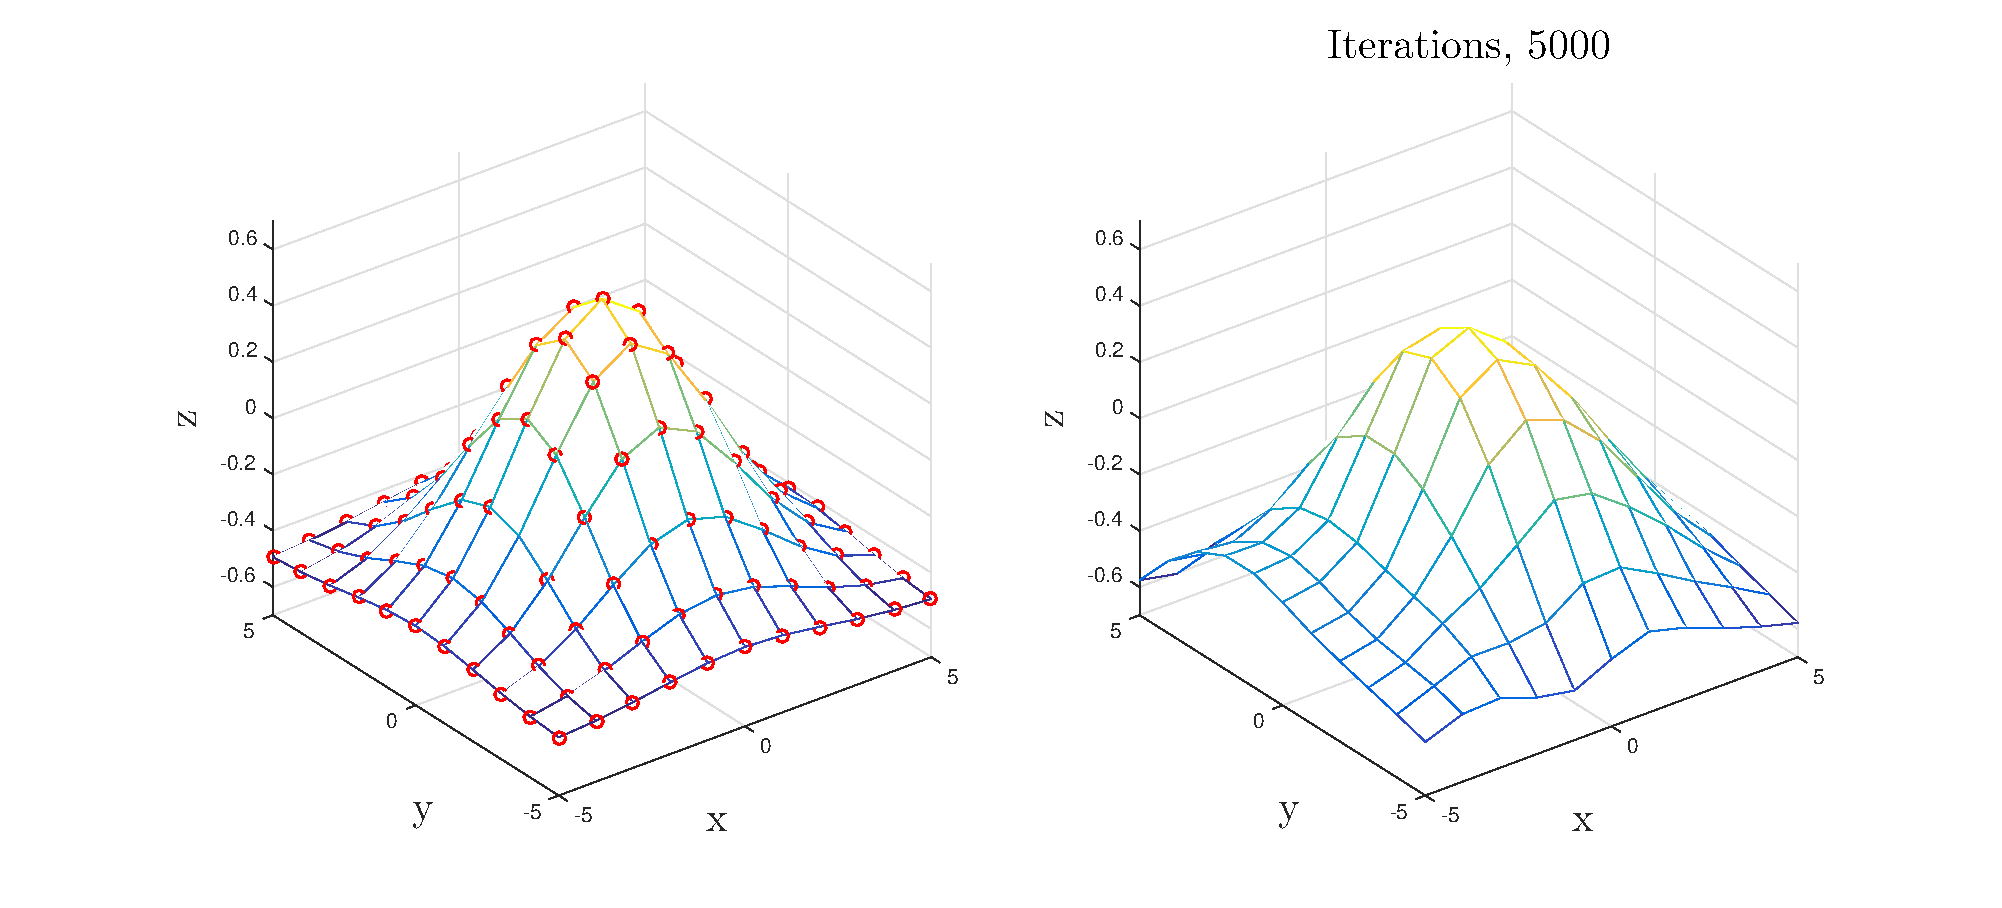
\includegraphics[width=\textwidth]{function_approximation_100}
        \caption{100 neurons in the hidden layer.}
        \label{fig:33}
    \end{subfigure}
    \caption{Neural network with one hidden layer approximates the given function $f(x,y)$ for different number of neurons in the hidden layer.}
    \label{f:3}
\end{figure*}

In addition, in Fig. \ref{fig:33} we observe that the results obtained with $100$ neurons is still OK. This is mainly due to the fact that the network drops the majority of the neurons in the hidden layer by setting their associated weights to zero, as shown by Fig. \ref{f:4}. 

\begin{figure}[h]
\centering
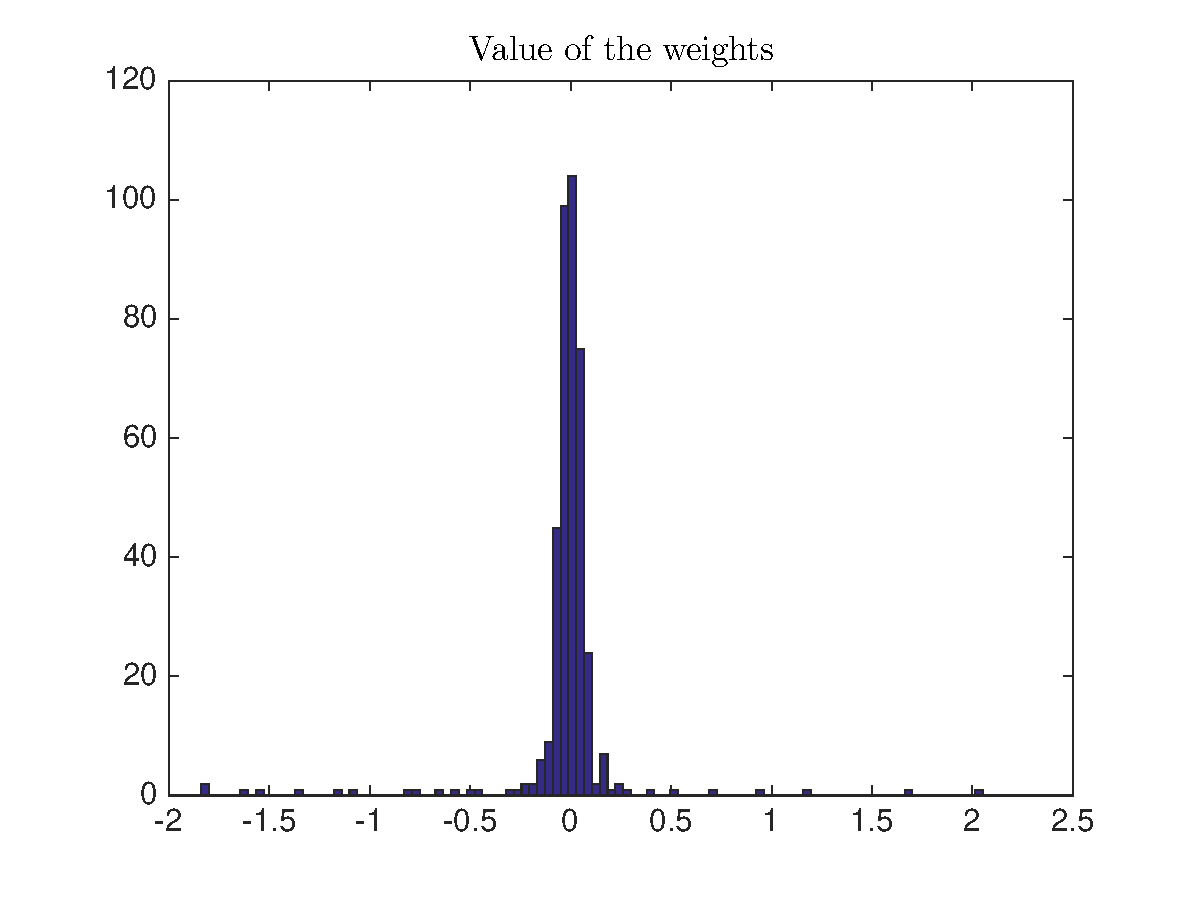
\includegraphics[scale=0.4]{function_approximation_100_hist}
\caption{Mean square error of the encoder.}
\label{f:4}
\end{figure}

If the inputs were affected by noise, we would not have that many weights approaching zero but rather all of them would try to account for the noisy perturbances. Thus, it would lead to overfitting and poor generalization of the estimation given by the neural network.

\section{GENERALIZATION}
Here we train the NN with a subselection of all the training points and evaluate it comparing to the underlying function, see Fig. \ref{f:5}.

\begin{figure}[h]
    \centering
    \begin{subfigure}[b]{0.45\textwidth}
        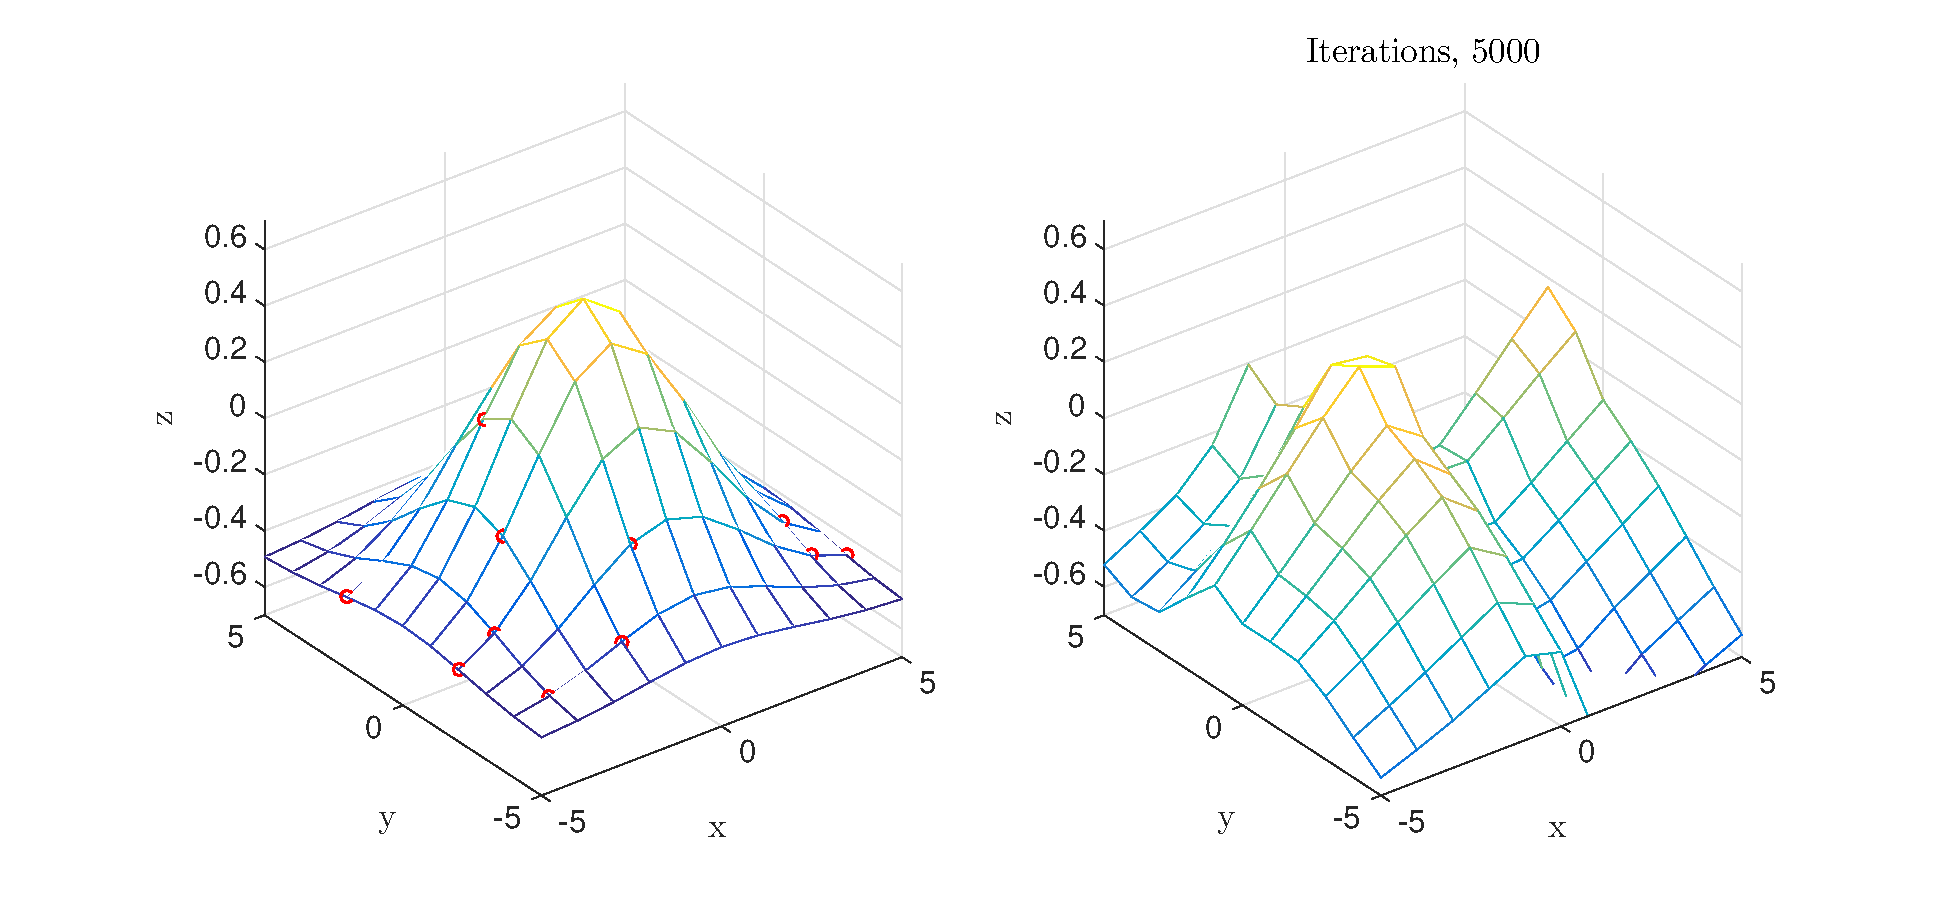
\includegraphics[width=\textwidth]{gene_15}
        \caption{15 training samples.}
        \label{fig:41}
    \end{subfigure}

    \begin{subfigure}[b]{0.45\textwidth}
        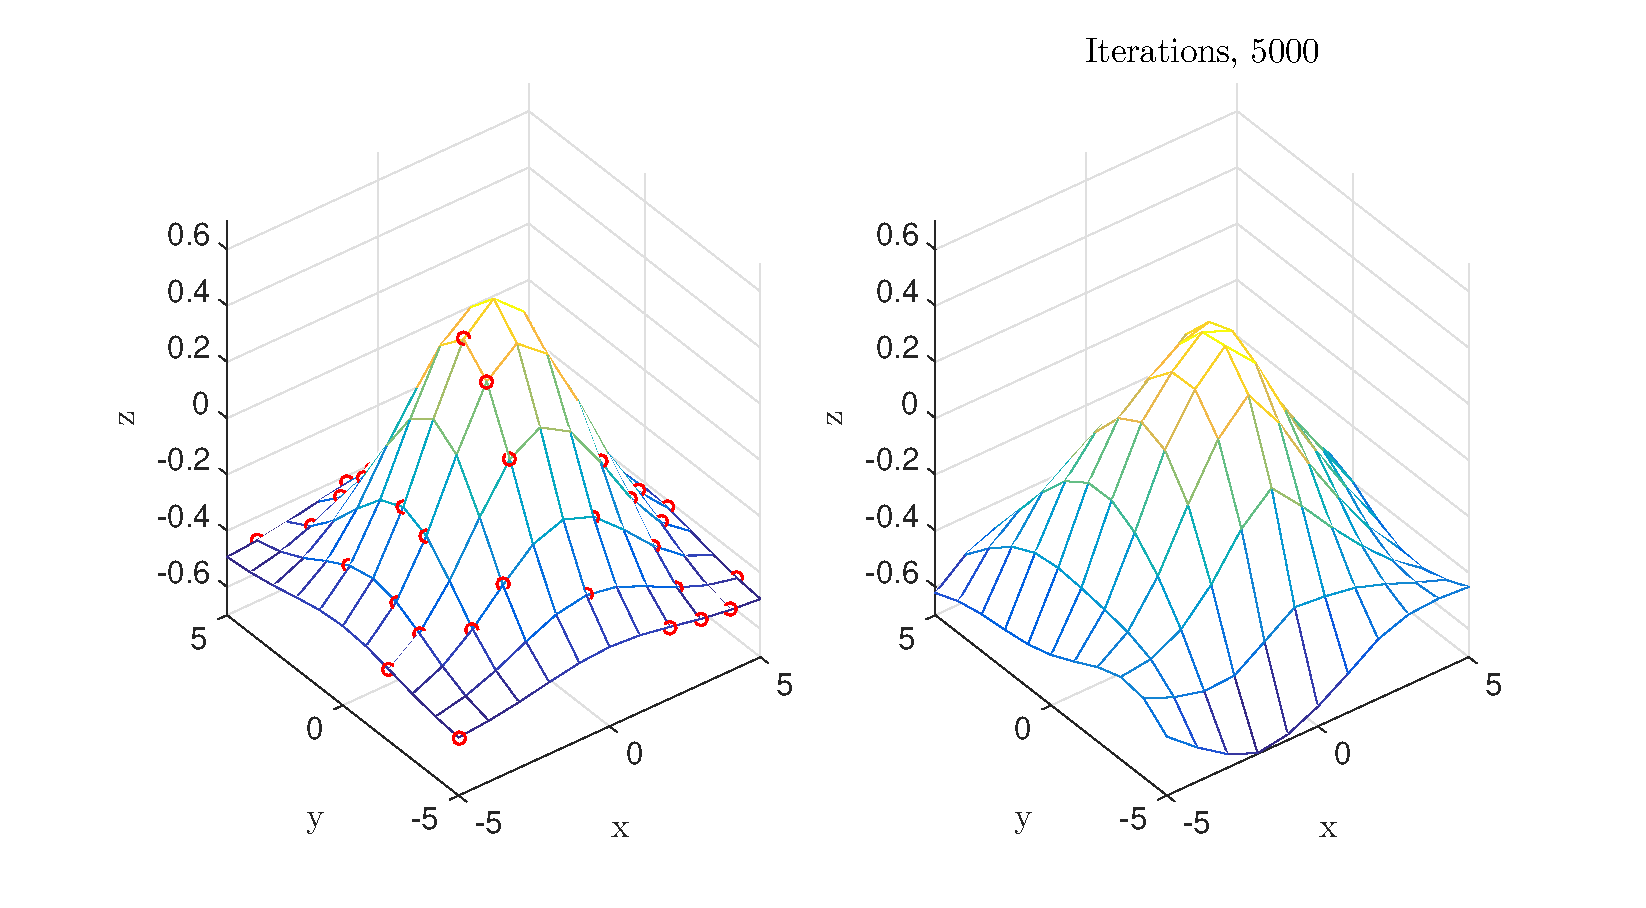
\includegraphics[width=\textwidth]{gene_40}
        \caption{40 training samples.}
        \label{fig:42}
    \end{subfigure}
    \caption{Estimation using different number of training samples. The whole set of training samples was of 125.}
    \label{f:5}
\end{figure}

\end{document}
